\documentclass{article}
\usepackage{indentfirst}
\usepackage{ctex}
\usepackage{geometry}
\usepackage{graphicx, subfigure}
\usepackage{enumerate}
\geometry{left=3.17cm,right=3.17cm,top=2.54cm,bottom=2.54cm} % 页边距

\begin{document}

\title{BigTable论文笔记}
\date{}
\maketitle

\section{Data Model(数据模型)}
BigTable集群是一个运行BigTable软件的进程集合。每个集群都为一组table提供服务。BigTable中的每个table都是一个稀疏的分布式持久化的多维有序map。数据以三个维度进行组织:行,列,时间戳。

\subsection{Rows}
BigTable按照行关键字的字典序组织数据。BigTable的行关键字为任意字符串。通过单个行关键字对数据的读写操作是可串行化的(不论当前行中的数据有多少不同的列正在被读写),这一设计使得客户端在面临针对同一行数据的并发更新时,能够更容易理解系统行为。换句话说,BigTable以“行”作为事务一致性的单位,目前不支持跨行事务。\par
拥有连续关键字的的行被组织成tablets,构成了数据分布和负载均衡的单位。这种数据组织方式使得读取小范围内的行更加高效,并且通常只需要和少数的机器进行通信。客户端可以通过选择特定的行关键字来利用这一特性,从而在数据访问中获得更好的局部性(locality)。

\subsection{Columns}
列关键字被组织成“列族(\emph{column families})”,构成了访问控制的单位。所有通过列族排序的数据通常是同类型的(我们把同一列族的数据一起进行压缩)。一个列族必须在该族中所有数据能够被存储在任意列关键字下之前就被显式创建。一个列族被创建后,改族的任意列关键字都可以被使用:数据可以存储在这样的列关键字之下,而不会影响到table的模式。我们的意图是,一个table中不同列族的数量要尽可能少(最多只能几百个),而且在数据操作期间几乎不去修改列族;这一限制很大程度上避免了元数据(metadata)变得过大。相反,一个table拥有的列关键字个数是不受约束的。\par
对整个列族的删除操作可以通过更改table的模式来完成,此时存储在那个列族中所有列关键字下的数据都会被删除。由于BigTable不支持跨行事务,如果存储在某个特定列关键字下的数据驻留在多个行中,那么它将不能被原子地删除。\par
列关键字的命名格式为:列族名:限定符(\emph{family:qualifier})。列族名必须是可打印的,但是限定符可以是任意字符串。

\subsection{Timestamps}
一个table中不同的cells可以包含同一数据的多个版本,版本信息通过时间戳进行索引。BigTable的时间戳是64-bit整数,它们由BigTable隐式赋值,代表“实时时间”的微秒值,也可由客户端应用程序显式赋值。需要避免崩溃的应用程序必须自己生成独一无二的时间戳。一个cell中不同版本的数据按照时间戳降序存储,使得最新版本的数据能被最先读取。\par
为了减轻多个版本数据的管理负担,我们对每一个列族配有两个设置参数,以此实现BigTable对多版本数据的自动垃圾回收。客户端可以指定只保存最后n个版本的数据,或者“足够新”的数据(比如只保存最近7天写入的记录)。

\section{Building Blocks(构件)}
BigTable是构建在其他几个Google基础组件之上的。BigTable集群通常运行在一个共享机器池中,这些机器上运行着各种分布式应用程序。BigTable依赖于Google集群管理系统,该系统负责共享机器的作业调度,资源管理,机器状态监控,以及机器故障处理。BigTable进程通常和其他应用程序进程共享相同的机器。\par
BigTable使用GFS存储日志和数据文件。GFS是一个分布式文件系统,它通过为每个文件维护多个副本的方式来实现更高的可靠性和可用性。\par
BigTable数据文件使用SSTable文件存储。SSTable实现了一种持久化、不可修改的有序KV映射结构,key和value都可以是任意字符串。SSTable提供了KV数据查询和遍历操作。SSTable包含了一组block序列(每个block的默认大小是64KB,但是大小是可配置的)。block index(存储在SSTable的末尾)用于定位block;当SSTable被打开时,index被载入内存。SSTable的查询操作是一次磁盘随机读:首先对内存中的index进行二分查找,找到合适的block,然后从磁盘读出相应的block。当然,也可以选择将整个SSTable映射到内存,这样就无需进行磁盘操作了。\par
BigTable依赖于一个高可用的持久化分布式锁服务Chubby。Chubby服务由5个活动副本组成,其中一个被选举为master,用于处理请求。只有在大多数副本正常运行,并且彼此能够正常通信的前提下,Chubby服务才是可用的。在面临故障时,Chubby使用Paxos算法保证副本一致性。Chubby提供了一个由文件夹和小文件组成的命名空间。每个文件夹和文件都可被用作一个锁,并且对每一个文件的读写是原子性的。Chubby客户端库提供了Chubby文件的一致性缓存。每个Chubby客户端都维持一个与Chubby服务的会话(session)。如果一个客户端会话无法在租期内重新签订会话租约,这个会话到期后就失效了。当客户端会话到期后,它将丢失持有的锁和打开的句柄。Chubby客户端也可以向Chubby文件和文件夹注册回调函数,一旦它们的状态发生改变,或者会话到期,Chubby客户端就可以得到通知。\par
BigTable使用Chubby实现各种任务:确保在任何时间都至少有一个活跃的master;存储BigTable数据的引导程序(bootstrap)的位置;发现tablet服务器,并在tablet服务器失效后采取措施;存储BigTable模式信息。如果Chubby长时间内不可用,BigTable就会失效。

\section{Implementation(实现)}
BigTable的实现包括3个主要组件:链接到客户端的库,一个master服务器,多个tablet服务器。为了适应工作负载的变化,可以向集群中动态添加(或删除)Tablet服务器。\par
master负责向tablet服务器分配tablets,检测新加入的或过期失效的tablet服务器,对tablet服务器进行负载均衡,对GFS中的文件进行垃圾回收。另外,master还负责处理模式变化,比如table和列族的创建/删除。\par
每个tablet服务器都管理着一组tablets(每个tablet服务器通常管理10到1000个tablets)。tablet服务器负责处理针对已加载的table的读写请求,以及在tablet变得过大时,对其进行分裂。\par
和其他许多single-master类型的分布式存储系统一样,客户端数据不会经过master:客户端直接与tablet服务器通信来完成读写请求。因为BigTable客户端在获取tablet位置信息时不依赖于master,所以BigTable客户端甚至无需与master通信。因此,在实际应用中master的负载是很轻的。\par
BigTable集群存储了许多tables,每个table由一组tablets组成,而每个tablet又包含了某个范围内的行的所有相关数据。初始时,每个table只拥有一个tablet。随着table的增长,它自动分裂成多个tablets,每个tablet的缺省大小为1GB。\par
虽然我们的模型支持任意大小的数据,但是当前的BigTable实现并不支持极其庞大的数据。由于tablet无法从一行的中间进行分裂,所以我们建议用户在一行内最多存储的数据量不要超过数百GB。\par
在本节接下来的内容中,我们会描述一些BigTable的实现细节。

\subsection{Tablet Location(Tablet的位置)}
我们使用一种类似于B+树的三层架构来存储tablet的位置信息(图\ref{fig:tablet_location_hierarchy})。第一层是一个存储在Chubby内的文件,保存了root tablet的位置信息。root tablet保存了METADATA表里的所有tablets的位置信息。每个METADATA子表保存了一组用户子表(user tablets)的位置信息。root tablet需要特殊对待——它永不分裂——以此保证tablet的位置层次结构不会超过3层。

\begin{figure}[htbp]
    \centering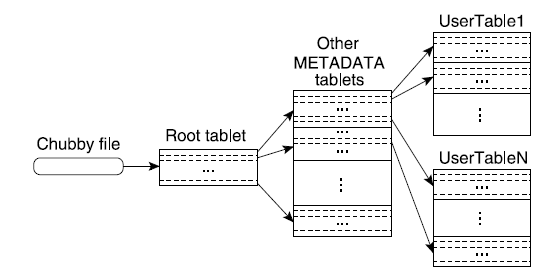
\includegraphics[height=5cm]{images/tablet_location_hierarchy.png}
    \caption{tablet location hierarchy}
    \label{fig:tablet_location_hierarchy}
\end{figure}

\par
METADATA表将tablet的位置信息存储在行关键字下,而这个行关键字是由tablet所属table的标识符和tablet的最后一行编码而成。METADATA的每一行存储了内存中大约1 KB的数据。在METADATA子表128 MB的保守存储限制下,采用这种三层位置存储模式足以标识$2^{34}$个tablets的位置。\par
客户端软件库通过遍历位置层次结构来定位tablets,然后缓存找到的tablets的位置信息。如果客户端不知道某个tablet的位置,或者发现它缓存的位置信息不正确,那么客户端就会递归地在树状层次结构中查询tablet的位置。如果客户端的缓存为空,定位算法就需要3次网络往返通信才能确定tablet的位置,包括对Chubby的一次读操作。如果客户端缓存过期了(stale),定位算法就需要6次往返通信(3次往返通信发现缓存过期,3次往返通信更新缓存),因为过期的缓存项只有在cache miss的时候才会被发现(我们期望这种情况不要太频繁,因为METADATA子表不应该被频繁地移动)。虽然tablet位置信息存储在内存中,因此对tablet的查询操作无需访问GFS,但我们仍可以通过在客户端软件库预取tablet位置来进一步减小开销:当客户端读取METADATA表的时候一次读出多条tablet的元数据。\par
我们也将次级信息(secondary information)存储在METADATA表,包括与每个tablet关联的所有事件日志(例如:一个tablet服务器何时启动为其提供服务)。这些信息对于调试和性能分析都非常有用。

\subsection{Tablet Assignment(Tablet分配)}
在任意时刻,每个tablet最多被分配给一个tablet服务器。master跟踪记录当前活跃的tablet服务器、tablets的分配情况,以及哪些tablets未被分配给tablet服务器。当一个tablet未被分配时,如果存在一个空间充足且可用的tablet服务器,master就向这个tablet服务器发送tablet加载请求(tablet load requests),从而将tablet分配给这个服务器。只有在下一个master故障转移之前tablet服务器未接受到tablet加载请求的情况下,这种分配才会失败:tablet服务器只接收来自当前master的tablet加载请求。因此,一旦master发送了tablet加载请求,它就有理由认为:直到tablet服务器失效前,tablet一直处于已被分配的状态;否则,tablet服务器通知master,它尚未加载tablet。\par
BigTable使用Chubby跟踪记录tablet服务器状态。当tablet服务器启动时,它会在一个特定的Chubby文件夹下新建一个唯一命名的文件,然后在这个文件上创建一个互斥锁并持有它。master通过实时监控该文件夹(服务器文件夹)的状态来发现新加入的tablet服务器。如果tablet服务器丢失了它的互斥锁,它就会停止对tablet提供服务:例如,网络分区可能会造成服务器丢失其Chubby会话。(Chubby提供了一种高效机制,允许tablet服务器在不引起网络拥塞的前提下检查自身是否还持有互斥锁。)只要文件还存在,tablet服务器就会尝试重新获得文件的互斥锁。如果文件不存在了,tablet服务器将无法再提供服务,于是它就会自行终止。无论tablet服务器何时终止(比如,因为集群管理系统从集群中移除该tablet服务器主机),它都会试图释放它所持有的锁,以便master能够快速地重新分配tablets。\par
master负责监控tablet何时不再为tablets提供服务,并尽快将那些tablets重新分配给新的tablet服务器。为了监控tablet服务器何时不再为tablets提供服务,master轮询每一个tablet服务器所持有的锁的状态。如果tablet服务器报告master它丢失了它的锁,或者master在经过数次尝试后仍无法连接到tablet服务器,master就会尝试获取该tablet服务器文件上的互斥锁。如果master能够获得该锁,就说明Chubby运行正常,而tablet服务器或是宕机,或是无法连接到Chubby,那么master就要通过删除tablet服务器在Chubby上的文件以确保它不再给tablet提供服务。一旦服务器文件被删除,master就将之前分配给该tablet服务器的tablets放进未分配的tablets的集合中。为了确保BigTable集群不受master和Chubby之间网络通信问题的影响,master在Chubby会话到期时自行终止。master的故障不会改变tablet在tablet服务器上的分配状态。\par
当master在集群管理系统中启动后,它必须先了解当前tablet的分配状态,然后才能改变分配状态。master启动时的执行步骤如下:
\begin{enumerate}[(1)]
	\item master在Chubby中获取一个唯一的\emph{master}锁,用来阻止并发的master实例。
	\item master扫描Chubby上的服务器文件夹,探知存活的服务器。
	\item master和所有tablet服务器通信,探知哪些tablets已经被分配给tablet服务器,并更新这些tablet服务器上记录的master状态信息(如果tablet服务器后续又接收到从先前的master发送来的tablet加载请求,它将拒绝这些请求)。
	\item master扫描METADATA表,学习tablets集合。如果扫描过程中遇到未分配的tablet,master就将其添加到未分配的tablets集合中以等待合适的分配时机。
\end{enumerate}

\par
一个复杂之处在于,只有等到所有METADATA子表被分配出去后,对METADATA表的扫描才得以进行。因此,在开始扫描之前(Step (4)),如果在Step (3)中发现root tablet处于未分配状态,master就把root tablet添加到未分配的tablets集合中,保证root tablet一定会被分配给tablet服务器。因为root tablet包含所有METADATA子表的名字,所以master完成对root tablet的扫描后便可知道它们的名字。\par
保存现有的tablets的集合只有在以下情形中会发生改变:创建或删除table,把两个现有的tablets合并成一个更大的tablet,或者把一个现有的tablet分裂成两个更小的tablets。master可以跟踪记录这些变化,因为除了最后一种情形,其余情形都是由master引发的。tablet分裂操作需要特殊处理,因为tablets的初始化是由tablet服务器完成的。tablet服务器在完成一次分裂操作后,通过在METADATA表里记录新的tablet的信息来提交本次操作。提交分裂操作之后,tablet服务器会通知master。如果通知信息丢失(tablet服务器或master宕机所致),master在要求tablet服务器加载刚分裂出来的新tablet之时,就会检测到这个新的tablet。由于tablet服务器在METADATA表中找到的tablet entry只是master要求它加载的tablet的一部分,它会将分裂操作通知给master(译者的理解:tablet在接受到master的tablet加载请求到执行请求的这段时间内,要求加载的tablet被分裂了,那么tablet服务器准备执行加载请求时就会发现,它只能找到该tablet的一部分,所以它就会向master发送tablet已被分裂的通知)。

\subsection{Tablet Serving(Tablet服务)}
\begin{figure}[htbp]
    \centering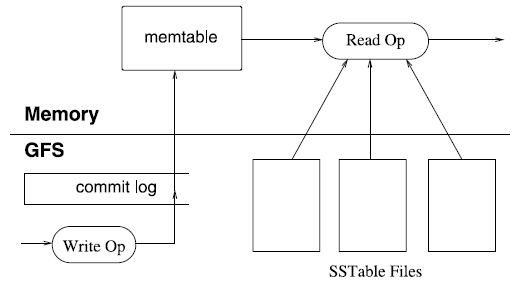
\includegraphics[height=5cm]{images/tablet_representation.png}
    \caption{tablet representation}
    \label{fig:tablet_representation}
\end{figure}

如图\ref{fig:tablet_representation}所示,tablet的持久化状态信息存储在GFS中。更新被提交至存储恢复记录(redo records)的提交日志(commit log)中。最近几次的已提交的更新存储在内存中名为\emph{memtable}的排序缓存中。memtable以行为单位维护这些更新,每一行使用copy-on-write机制保持行级(row-level)一致性。旧的更新存储在一系列不可修改的SSTable中。\par
tablet服务器通过从MATADATA表读取tablet元信息来恢复tablet。这些元信息包括组成tablet的SSTable列表,以及一组恢复点(redo points),这些redo points指向任何可能包含tablet数据的提交日志。服务器把SSTables的索引读入内存,应用redo points之后以提交的更新,以此重建memtable。\par
当写操作到达tablet服务器时,服务器检查其格式是否正确,以及写者是否有执行该操作的权限——有一个Chubby文件保存了拥有写权限的操作者列表,tablet服务器通过读取该文件即可验证某个写者是否拥有写权限。对于有效的写操作,服务器将其记录到提交日志中。可以采用批量提交来提高包含大量小的修改操作的客户端的吞吐量。写操作被提交后,写的内容就会被插入到memtable。\par
当读操作到底tablet服务器时,类似与写操作,服务器检查其格式和权限。一个有效的读操作在一系列SSTables和memtable的合并视图(merged view)中执行。由于SSTables和memtable都是基于字典序的数据存储结构,所以可以高效地构建合并视图。\par
当tablets正在被分裂或合并时,新到来的读写操作都是能够正常继续的。当tablets正在被压缩的时候,读写操作也是可能会出现的;压缩的具体内容在下一节讲述。

\subsection{Compactions(压缩)}
随着写操作的进行,memtable的大小不断增加。当memtable的大小达到阈值时,就将其冻结并创建一个新的memtable,然后被冻结的memtable被转换为SSTable并写入GFS。该过程称为\emph{minor compation},其目标有二:缩减tablet服务器的内存占用;如果服务器宕机,可以减少服务器恢复期间需从提交日志中读取的数据量。\par
每次minor compaction都会创建一个新的SSTable。如果minor compation一直得不到检查,读操作可能需要合并来自多个SSTables的更新。因此,我们通过在后台周期性地执行\emph{merging compaction}来限制此类SSTables的数量。merging compaction读取若干SSTables和memtable,将其重新写入一个新的SSTable。merging compaction结束后,作为输入的SSTables和memtable立即被废弃。\par
将所有SSTables重新写入一个SSTable的merging compaction称为\emph{major compaction}。由non-major compactions生成的SSTables可能包含特殊的删除项,这些删除项隐藏了仍存在于旧SSTables中的已删除的数据。换句话说,major compaction生成的SSTables中不包含删除信息或已删除的数据(译者记:结合LevelDB,删除都是标记删除,真正的删除发生在major compaction合并SSTables之时)。BigTable轮询所有tablets,定期对其执行major compaction。这些major compaction使得BigTable得以回收那些被标记删除的数据占用的资源,保证被标记删除的数据及时从系统中消失——这对于存储敏感数据的服务而言很重要。\par
BigTable优异的读性能得益于GFS的局部性优化。写文件的时候,GFS尝试在同一个写者机器上放置一份数据副本。读文件的时候,由距读者最近的一个文件副本提供服务。因此,在tablet服务器和GFS服务器共享主机的通常情况下,tablet服务器会把数据压缩到SSTables,并在本地磁盘上为其创建一个副本,以此来保证后续针对SSTables的读请求能够被快速处理。

\subsection{Schema Management(模式管理)}
BigTable模式信息存储在Chubby中。Chubby为BigTable模式提供了有效的通信基础组件,因为它提供了针对整个文件的原子写操作,以及小文件的一致性缓存。例如,假设客户端想删除一个table的列族中的某些列。master执行访问控制检查,并在客户端的删除操作结束后检查模式的格式正确性,然后通过重写Chubby中相应的模式文件来建立新模式。不管tablet服务器何时需要确定当前有哪些列族,它只需从Chubby读取相关的模式文件即可,这些文件存在于服务器的Chubby客户端缓存中,并且几乎总是可用的。因为Chubby缓存的一致性,文件的所有更改都对tablet服务器可见。

\section{REFINEMENTS(优化)}
上一节中描述的BigTable实现需要做一些优化才能达到用户要求的高性能、高可用和高可靠性。为了强调这些优化内容,本节将从细节上更加深入地描述BigTable的部分实现。

\subsection{Locality Groups(局部性群组)}
每一个列族都被分配给一个客户端自定义的局部性群组——一个能让客户端控制其数据存储布局的抽象描述。在compaction期间,对于tablet中的每个局部性群组都会单独生成一个SSTable。将通常不会一起访问的列族隔离到单独的局部性群组中可以提高读操作的效率。\par
另外,可以为每个局部性群组制定一些有用的配置参数(tuning parameters)。例如:可以将一个局部性设定为存储在内存中。对于内存中的局部性群组而言,SSTables以延迟加载的方式加载到tablet服务器内存中。由于SSTables是不可更改的,所以不存在一致性问题。一旦加载完毕,读取局部性群组中的列族时就不必访问磁盘了。这一特性对于小块数据的频繁访问是很有用的;we use it internally for the tablet-location column family in the METADATA tablet.

\subsection{Compression(压缩)}
客户端可以控制是否需要对一个局部性群组的SSTables进行压缩,并指定压缩格式。用户指定的压缩格式会被应用到每一个SSTable的block(通过局部性群组的配置参数可以控制block的大小)。单独压缩每一个block会损失一些磁盘空间(译者注:分块压缩的压缩比率要比整体压缩的低),但是我们无需解压缩整个文件便可读取SSTable的一小部分数据。许多BigTable客户端使用的是两趟自定义压缩模式。第一趟使用Bentley and Mcllroy's模式,对一个大窗口中的长公共字符串(long common strings)进行压缩。第二趟使用一种快速压缩算法,该算法在一个包含16KB数据的小窗口中搜索重复数据。两趟压缩都是极快的——在现代机器上,编码速率可达100-200MB/s,解码数据可达400-1000MB/s。\par
尽管我们在选择压缩算法时强调速度而不是空间,但是上述的两趟压缩模式在这两点上都异常出色。比如在Webtable中,我们使用该压缩模式来存储网页内容。在一次实验中,我们在一个经过压缩的局部性群组中存储了大量的文档。出于实验目的,我们在存储文档时存储了对我们可用的一个版本,而非全部版本。该模式实现了10:1的空间压缩比,明显优于传统Gzip针对HTML页面的3:1或4:1的压缩比,这得益于Webtable的行数据布局方式:来自单个主机的页面彼此紧邻存储。这使得Bentley-Mcllroy算法能够识别出来自同一个主机的网页中的大量重复内容。许多应用程序,不只是BigTable,在选择行关键字的时候都尽可能让相似的数据聚集在一起,因此能够实现非常理想的压缩比率。如果我们在BigTable中存储相同数据的多个版本,则可获得更高的压缩比率(译者注: 利用BigTable的timestamp,可以存储相同数据的多个版本)。

\subsection{Caching for Read Performance(通过缓存技术提高读操作的性能)}
tablet服务器使用两级缓存来提高读操作的性能。Scan Cache是一级缓存,缓存的是tablet服务器通过SSTable接口返回的key-value对。Block Cache是二级缓存,缓存的是从GFS读入的SSTable的blocks。Scan Cache对于经常反复读取相同数据的应用程序来说非常有用。Block Cache对于经常读取和最近读取的数据临近的数据的应用程序来说非常有用(比如,针对一个hot row中的相同局部性群组的不同列的顺序读(sequential reads)或随机读(random read))。

\subsection{Bloom Filters}
一次读操作必须读取构成一个tablet状态的所有SSTables。如果这些SSTables尚未装入内存,我们可能需要进行多次磁盘访问。通过让客户端为特定的局部性群组中的SSTables指定Bloom Filters,我们就能够减少磁盘访问次数。Bloom Filter允许我们询问一个SSTable是否包含指定的行/列数据对。对于特定的应用程序,只需在tablet服务器内存中开辟一小块空间来存储Bloom Filters,就可以大幅减少读操作所需要随机磁盘访问。Bloom Filters的使用亦可避免大多数针对不存在的行/列数据的查询而导致的磁盘访问。

\subsection{Commit-Log Implementation(提交日志的实现)}
如果我们为每个tablet的提交日志都保存为一个日志文件,就需要在GFS中对大量文件进行并发写。基于每个GFS服务器的底层文件系统实现,这些写操作可能需要大量的磁盘随机访问才能写入不同的磁盘日志文件。另外,由于批量提交(group commit)的操作数目一般比较小,为每个tablet设置单独的日志文件也会降低批量操作本应具有的效率。为了解决这些问题,我们把每一个tablet服务器的修改日志都已追加方式写入同一个提交日志中,这样一来,同一个日志文件中就混杂了不同tablet服务器的修改操作的日志记录。\par
对于常规操作而言,仅适用一个日志文件无疑带来了极高的性能突破,但这使得恢复操作复杂化。当tablet服务器宕机时,它所服务的tablets会被重新分配到大量其他的tablet服务器;这些服务器一般只会加载最初宕机的服务器上的少数tablets。为了恢复某个tablet的状态,新的tablet服务器需要重新从最初宕机的服务器写入的提交日志中为该tablet应用修改记录。然而,这些tablets的修改日志是混杂在同一个磁盘文件中的。一种方案是,每个新的tablet服务器读入完整的提交日志,但是仅应用那些需要用于恢复它所加载的tablets的日志项。然而在该模式下,如果100台机器中每台只从宕机服务器那里分配到一个tablet,那么就需要读取同一个日志文件100次(每个服务器读一次)。\par
我们通过提交日志项的key<table, row name, log sequence number>对日志项进行排序,以此避免对同一日志文件的重复读。在排序输出结果中,对于特定tablet的所有修改记录都是连续的,因此可以在一次磁盘随机读之后进行顺序读,从而提高读性能。为了实现排序的并行化,我们把日志文件分成多个64MB的片段,在不同的tablet服务器上对每个片段并行排序。排序进程由master进行调度;当一个tablet服务器需要从提交日志文件中恢复对tablets的修改操作时,排序进程即刻启动。\par
由于各种原因,在GFS中写提交日志有时会产生性能瓶颈(比如,GFS服务器主机发生了写操作崩溃,负载过高,与一组特定的GFS服务器之间的网络通信受阻)。为了让修改操作避开GFS服务器的延迟峰值,每个tablet服务器配有两个写线程,每个线程都只写自己的日志文件;在任意时刻只有一个线程出入活跃状态。如果一个线程对日志文件的写性能明显下降,就切换到另一个线程,在提交日志队列中的修改操作由当前活跃的线程写入日志。日志项包含的序列号允许恢复线程忽略重复日志项——这是由线程切换产生的。

\subsection{Speeding Up Tablet Recovery(加速Tablet恢复)}
卸载tablet之前,tablet服务器首先对tablet做一个minor compaction,减少了服务器的提交日志中未压缩的日志项,从而减小了后续的恢复时间。完成minor compaction之后,tablet服务器就停止为tablet提供服务。在tablet服务器真正卸载tablet之前,它会再做一次minor compation(通常很快),清除服务器日志中尚未压缩的残留数据,这些数据是第一次minor compaction执行期间到达服务器的。第二次minor compaction完成后,tablet就能够被加载到另一个tablet服务器而无需恢复任何日志项。\par

\subsection{Exploiting Immutability}
除了SSTables缓存,BigTable系统的其他各部分都已得到简化,这是基于这样一个事实——SSTables一经生成就不再修改。例如,读取SSTables时无需对文件系统的访问进行任何同步(译者注:对同一文件的并发读不需要同步)。所以,我们可以高效地实现基于行(row)的并发控制。唯一可被修改的数据结构——可读可写——是memtable。为了减少memtable的读竞争,我们为memtable的每一行设置copy-on-write,使得读写得以并发执行。\par
由于SSTable不可修改,“永久移除标记删除的数据”这一问题就转变为对废弃的SSTables进行垃圾回收的问题了。每个tablet的SSTables信息都注册在METADATA表内。master在移除废弃的SSTables时,采用“标记-清除(mark-and-sweep)”的垃圾回收方式,METADATA表保存了这些SSTables的根节点信息。\par
最后,SSTables不可修改的特性让我们能够快速分裂tablets。与其为每一个新分裂出来的tablets(child tablets)生成一组新的SSTables,我们不如让这些新tablets与原来的tablet(parent tablet)共享SSTables。

\end{document}